\chapter{Correlation effects in attosecond electron dynamics} % (fold)
\label{cha:electron_correlation}

%%%%%%%%%%%%%%%%%%%%%%%%%%%%%%%%%%%%%%%%%%%%%%%%%%%%%%%%%%%%%%%%%%%%%%%%%%%%%%%%%%%%%%%%%%%%%%%%%%%%%%%%%%%%%%%%%%
%%%%%%%%%%%%%%%%%%%%%%%%%%%%%%%%%%%%%%%%%%%%%%%%%%%%%%%%%%%%%%%%%%%%%%%%%%%%%%%%%%%%%%%%%%%%%%%%%%%%%%%%%%%%%%%%%%
%%%%%%%%%%%%%%%%%%%%%%%%%%%%%%%%%%%%%%%%%%%%%%%%%%%%%%%%%%%%%%%%%%%%%%%%%%%%%%%%%%%%%%%%%%%%%%%%%%%%%%%%%%%%%%%%%%
%%%%%%%%%%%%%%%%%%%%%%%%%%%%%%%%%%%%%%%%%%%%%%%%%%%%%%%%%%%%%%%%%%%%%%%%%%%%%%%%%%%%%%%%%%%%%%%%%%%%%%%%%%%%%%%%%%
%%%%%%%%%%%%%%%%%%%%%%%%%%%%%%%%%%%%%%%%%%%%%%%%%%%%%%%%%%%%%%%%%%%%%%%%%%%%%%%%%%%%%%%%%%%%%%%%%%%%%%%%%%%%%%%%%%
\section{Hyperspherical harmonics}
\label{sec:hyperspherical}

Solving the TDSE for two active electrons is a computationally difficult task. A Naive approach would be to discretized the 6 spacial dimensions using finite difference. Finite difference would provide a straight forward solution and runs well on supercomputing systems, however, the size of the wavefunction scales like $N^6$. Therefore if we were to us a typical grid of 1000 points in each dimension, the wavefunction would be $10^{18}$ points in size. Merely writing down the wavefunction in double precision floating point numbers would require 16 Exabytes of RAM, approximately 100 times more RAM than exists on the largest supercomputer in the world (Summit, OLCF). Instead, it is convent to choose a basis that greatly reduces the size of the problem. One common approach is to use bi-spherical harmonics. In this case, each electron is expanded in 3D spherical coordinates. The radius is discretized with finite difference, b-splines, FEDVR, or similar method, and the two angular coordinates are explained in the standard 3D spherical harmonics in the same way a single active electron code would do. When taking the tensor product of the two electrons, the electron-electron repulsion term is then expanded in spherical harmonics such that
\begin{equation}
    \frac{1}{|\mathbf{r}_1-\mathbf{r}_2|}= 4\pi \sum_{\ell=0}^\infty \sum_{m=-\ell}^{m=\ell}\frac{1}{2\ell+1}\frac{r_<^\ell}{r_>^{\ell+1}}Y_{\ell m}^*(\theta_1, \phi_1)Y_{\ell m}^(\theta_2, \phi_2).
\end{equation}
Resulting in a 6D space that can be used to solve the problem of two electrons in a molecular or atomic potential interacting with a laser.

In the bi-spherical codes, one must discretize two radi. As the grid increases in size, the code likes $N^2$. To cercomvent this problem, I have implemented a code that contains a single hyper-radius ($R$) and five angles that are expanded in 6D hyperspherical harmonics. Therefore as the grid size is increased, the code scales like $N$ and the number of spherical harmonics is controlled by the laser parameters. In the following section, I will describe the details to implementing two different ``coordinate systems'' that solve the two active electron problem. The first is through the use of Jacobi Coordinates, which allows for the finite mass of the nucleus to be accounted for. The second is making the infinite mass approximation for the nucleus allowing for the distance between the two electrons to be accessed more directly. The two problems can be solved with similar sized wavefunctions, however, the second method has a greatly reduced time in calculating matrix elements. This section is laid out $\cdots$ \textbf{TODO}

\subsection{TDSE in hyperspherical coordinates} % (fold)
\label{sub:tdse_in_hyperspherical_coordinates}
The TDSE
\begin{equation}
    i\frac{\partial}{\partial t}\Psi = \hat{H}\Psi
\end{equation}
with hamiltonian written in hyperspherical coordinates is
\begin{equation}
   \hat{H} = -\frac{1}{2} \left[\frac{1}{R^5}\frac{\partial}{\partial R}\left(R^5\frac{\partial}{\partial R}\right) - \frac{\hat{K}^2(\Omega_5)}{R^2}\right] + \frac{W(\Omega_5)}{R}
\end{equation}
where $R=\sum_i x_i^2$ is the hyper radius with $x_i$ being a Cartesian coordinate, $\hat{K}$ as the angular momentum operator, $\Omega_5$ is the solid angle in 6D (5 angles), and $V(\mathbf{R}) = W(\Omega_5)/R$ being the potential. I will use the hyperspherical harmonics such they contain two-3D sub spaces as discribed in Sec.~\ref{ssub:spherical_harmonics}. 
The resulting volume elements are 
\begin{equation}
    d\tau = R^5 dr d\Omega_i
\end{equation}
\begin{equation}
    d\Omega_i = \cos^2\alpha \sin^2\alpha d\alpha d\omega
\end{equation}
\begin{equation}
    d\omega = \sin\theta_{r_1} d\theta_{r_1} d\phi_{r_1} \sin\theta_{r_1} d\theta_{r_1} d\phi_{r_1}
\end{equation}
where $\theta_i$ and $\phi_i$ denote the angles in the $i={r_1}$ and $i={r_1}$ sub coordinate systems and $\alpha$ is the angle produced by the right triangle with sides R, ${r_1}$, and ${r_1}$ as shown in Fig.~\ref{fig:hyperradius}. $r_1$ and $r_2$ will be used as the Jacobi Coordinates for finite mass nucleus is considered or the single electron coordinates when the infinite mass approximation is made.
\begin{figure}[h!]
\centering
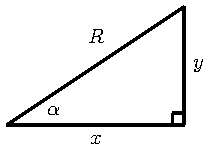
\includegraphics[width=0.3\linewidth]{figs/Two_electron/hyperradius.pdf}
\caption{How the hyperradius (R) relates to the two single-electron sub coordinate systems ($r_1$, $r_2$)} 
  \label{fig:hyperradius}
\end{figure}

As with the 3D TDSE, it is beneficial to remove the first derivative in the radial equation. This is accomplished by making a substitution of $\Psi = \psi/R^{5/2}$ giving us a Hamiltonian
\begin{equation}
   \hat{H} = -\frac{1}{2} \left[\frac{\partial^2}{\partial R^2} - \frac{\hat{K}^2(\Omega_5)+15/4}{R^2}\right] + \frac{W(\Omega_5)}{R}.
\end{equation}
The wavefunction can now be written as
\begin{equation}
    \psi = \sum\limits_{\mathbf{K}} U_{\mathbf{K}}(R) Y_{\mathbf{K}}(\Omega_5)
\end{equation}
with $U_{\mathbf{k}}(R)$ being the hyperradial part of the wavefunction and $Y_{\mathbf{K}}(\Omega_5)$ being the 6D hyperspherical harmonics described in Sec.~\ref{sec:spherical_harmonics}. Since hyperspherical harmonics are eigenfunctions of $\hat{K}^2$ with eigenvalue $K(K+4)$, the Hamiltonian becomes
\begin{equation}
   \hat{H}_{K} = -\frac{1}{2} \left[\frac{\partial^2}{\partial R^2} - \frac{K(K+4)+15/4}{R^2}\right] + \frac{W(\Omega_5)}{R}.
\end{equation}
I solve this equation using finite difference to discretized the hyperradial function ($U_{\mathbf{K}}(R)$). By setting $W(\Omega_5)=1$, the equation is the 6D hydrogen atom with an analytic solution that can be used to test the hyperadial portion of the code (see \cite{S_revik_2005} for energy levels). The angular portion of the equations is then expanded in hyperspherical harmonics. The details of the expansion are the focus of the remainder of this section.
% subsection tdse_in_hyperspherical_coordinates (end)

\subsubsection{Hyperspherical Harmonic Definition} % (fold)
\label{ssub:spherical_harmonics}
Utilizing Jacobi coordinates with $\mathbf{x_1}$ being the coordinate between the two electrons and $\mathbf{y_1}$ being the coordinate between the center of mass of the $e^-e^-$ pair and the nucleus. Our system is now a 6D space that we will describe by a hyper radius ($R$) and 5 angles contained in the solid angle $\Omega_{5_1}$. The angles will be expanded in 6D Hyperspherical harmonics that can be written in Jacobi coordinate system 1 as
\begin{align}
    Y^{\ell_{x_1},\ell_{y_1}}_{K,L,M}(\Omega_{5_1}) =& N^{\ell_{x_1},\ell_{y_1}}_K P_n^{(\ell_{x_1}+1/2,\ell_{y_1}+1/2)}(\cos(2\alpha)) \cos^{\ell_{x_1}}(\alpha) \sin^{\ell_{y_1}}(\alpha) \\ 
    &\times\sum_{m_x,m_y}\bra{L,M}\ket{\ell_{x_1},m_x,\ell_{y_1},m_y}  \left[Y_{\ell_{x_1},m_x}(\hat{x}_1)\times Y_{\ell_{y_1},m_y}(\hat{y}_1)\right]
\end{align}
with
\begin{equation}
    N^{\ell_x,\ell_y}_K = \sqrt{\frac{2(K+2)(n!)\Gamma (n+\ell_x+\ell_y+2)}{\Gamma (n+\ell_x+3/2) \Gamma (n+\ell_y++3/2)}}
\end{equation}
where $P_n^{(\alpha,\beta)}$ is a Jacobi polynomial, $\bra{L,M}\ket{\ell_{x_1},m_x,\ell_{y_1},m_y}$ is a Clebsch–Gordan coefficient, and $\Gamma$ is a gamma function. 
The quantum numbers are $K,\ell_{x_1},\ell_{y_1},L,M$ with $K=2n+\ell_{x_1}+\ell_{y_1}$ being the grand angular momentum, $\ell_{x_1}\ge0$ and $\ell_{y_1}\ge0$ being the angular momentum for the $\mathbf{x_1}$ and $\mathbf{y_2}$ coordinates respectively, $|\ell_{x_1}-\ell_{y_1}|\le L \le \ell_{x_1}+\ell_{y_1}$ and $-L \le M \le L$.

It is convenient to separate out the part that depends on $\alpha$ from the $\mathbf{x}$ and $\mathbf{y}$ portions. We define
\begin{equation}
    \tilde{P}^{\ell_{x_1},\ell_{y_1}}_{n}(\alpha) = N^{\ell_{x_1},\ell_{y_1}}_K P_n^{(\ell_{x_1}+1/2,\ell_{y_1}+1/2)}(\cos(2\alpha)) \cos^{\ell_{x_1}}(\alpha) \sin^{\ell_{y_1}}(\alpha) 
\end{equation}
making the spherical harmonics 
\begin{equation}
    Y^{\ell_{x_1},\ell_{y_1}}_{K,L,M}(\Omega_{5_1}) =\tilde{P}^{\ell_{x_1},\ell_{y_1}}_{n}(\alpha)\sum_{m_x,m_y}\bra{L,M}\ket{\ell_{x_1},m_x,\ell_{y_1},m_y}  \left[Y_{\ell_{x_1},m_x}(\hat{x}_1)\times Y_{\ell_{y_1},m_y}(\hat{y}_1)\right].
\end{equation}
% section spherical_harmonics (end)
 
\subsubsection{Jacobi Coordinates} % (fold)
\label{ssub:jacobi_coordinates}
For many particle systems, it is convenient to define Jacobi coordinates

\begin{equation}
\mathbf{R_{cm}} = m_1 \mathbf{r_1} + m_2 \mathbf{r_2} + m_3 \mathbf{r_3}
\end{equation}
\begin{align}
\label{eq:jacobi_coords}
\mathbf{x_1} &= \left[\frac{m_2+m_3}{m_1(m_2+m_3)^2}\right]^{1/4} (\mathbf{r_3}-\mathbf{r_2}); &\mathbf{y_1} &= \left[\frac{m_1(m_2+m_3)^2}{m_2+m_3}\right]^{1/4} \left(\mathbf{r_1}- \frac{m_2\mathbf{r_2}+m_3\mathbf{r_3}}{m_2+m_3} \right)\\
\mathbf{x_2} &= \left[\frac{m_3+m_1}{m_2(m_3+m_1)^2}\right]^{1/4} (\mathbf{r_1}-\mathbf{r_3}); &\mathbf{y_2} &= \left[\frac{m_2(m_3+m_1)^2}{m_3+m_1}\right]^{1/4} \left(\mathbf{r_2}- \frac{m_3\mathbf{r_3}+m_1\mathbf{r_1}}{m_3+m_1} \right)\\
\mathbf{x_3} &= \left[\frac{m_1+m_2}{m_3(m_1+m_2)^2}\right]^{1/4} (\mathbf{r_2}-\mathbf{r_1}); &\mathbf{y_3} &= \left[\frac{m_3(m_1+m_2)^2}{m_1+m_2}\right]^{1/4} \left(\mathbf{r_3}- \frac{m_1\mathbf{r_1}+m_2\mathbf{r_2}}{m_1+m_2} \right)
\end{align}
The three coordinate systems are depicted in Fig.~\ref{fig:jacobi_coord}. For the Helium atom we place the nucleus as $m_1$ and the two electrons at $m_2$ and $m_3$. The we set $m_1\rightarrow \infty$ and $m_2=m_3=m$. Now we define $\beta_i$ with $i=1,2,3$ such that
\begin{align}
\mathbf{x_1} &= \beta_1 (\mathbf{r_3}-\mathbf{r_2}); \; \; \mathbf{y_1} = \frac{1}{\beta_1} \left(\mathbf{r_1}- \frac{\mathbf{r_2}+\mathbf{r_3}}{2} \right)\\
\mathbf{x_2} &= \beta_2 (\mathbf{r_1}-\mathbf{r_3}); \; \; \mathbf{y_2} = \frac{1}{\beta_2} \left(\mathbf{r_2}- \frac{\mathbf{r_3}+\mathbf{r_1}}{2} \right)\\
\mathbf{x_3} &= \beta_3 (\mathbf{r_2}-\mathbf{r_1}); \; \; \mathbf{y_3} = \frac{1}{\beta_2} \left(\mathbf{r_3}- \frac{\mathbf{r_1}+\mathbf{r_2}}{2} \right)
\end{align}
Within the infinite mass approximation, $\beta_1=1/\sqrt{2}$ and $\beta_2=\beta_3=1$. By applying a Raynal-Revai Coefficient (RRC, Sec.~\ref{ssub:raynal_revai_coefficient}) it is possible to transition between the three different coordinate systems.  The transformation conserves the angular momentum quantum numbers $K$ , $L$, and $M$.

\begin{figure}[t]
\centering
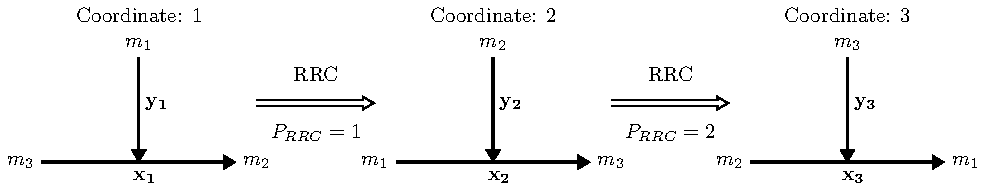
\includegraphics[width=\linewidth]{figs/Two_electron/coord_1.pdf}
\caption{The Jacobi coordinates for three body interactions. Each coordinate can be obtained from the previous by utilizing a Raynal-Revai Coefficient (RRC, Sec.~\ref{ssub:raynal_revai_coefficient})} 
  \label{fig:jacobi_coord}
\end{figure}

% section jacobi_coordinates (end)



\subsubsection{Raynal-Revai Coefficient (RRC)} % (fold)
\label{ssub:raynal_revai_coefficient}
The RRC coefficients for rotating between coordinate system $i$ and $j$ can be written explicitly as
\begin{align}
\nonumber
    <\ell_{x_j},\ell_{y_j}|\ell_{x_i},\ell_{y_i}>_{K,L} =& \frac{(-1)^{n_i+n_j}}{\sqrt{C_{\ell_{x_j}\ell_{y_j}}^{n_j}C_{\ell_{x_i}\ell_{y_i}}^{n_i}}} \sum\limits_{\lambda_1,\lambda_2,\lambda_3,\lambda_4} i^{\lambda_2-\lambda_1+\ell_{y_i}-\ell_{y_j}}\left[\prod_{k=1}^4 (2\lambda_k +1)\right] \\ 
\nonumber
    & \times \braket{\lambda_1 0 \lambda_3 0}{\ell_{x_j} 0} \braket{\lambda_2 0 \lambda_3 0}{\ell_{x_i} 0} \braket{\lambda_2 0 \lambda_4 0}{\ell_{y_j} 0} \braket{\lambda_1 0 \lambda_4 0}{\ell_{y_i} 0} \\
\nonumber
    & \times sgn(a_{12})^{\lambda_1}sgn(a_{21})^{\lambda_2}sgn(a_{11})^{\lambda_3}sgn(a_{22})^{\lambda_4} \begin{bmatrix}
   \lambda_3 & \lambda_1 & \ell_{x_j} \\
   \lambda_2 & \lambda_4 & \ell_{y_j} \\
   l_{x_i}   & l_{x_y}   & L
   \end{bmatrix} \\
    & \times \sum\limits_{\nu,\mu} (-1)^{\mu}|a_{12}|^{2\mu + \lambda_1 + \lambda_2} |a_{12}|^{2\nu + \lambda_3 + \lambda_4} C_{\lambda_1 \lambda_2}^{\mu} C_{\lambda_3 \lambda_4}^{\nu}
\end{align}
where $sgn(a_{ij})$ is the sign of $a_{ij}$, the sum is restricted by $K=2n_i+\ell_{x_i}+\ell_{y_i}=2n_j+\ell_{x_j}+\ell_{y_j}=2(\mu+\nu)+\lambda_1+\lambda_2+\lambda_3+\lambda_4$, $\braket{\lambda_1 0 \lambda_3 0}{\ell_{x_j} 0}$ is a Clebsch Gordan coefficient, 
% \begin{equation*}
     $\begin{bmatrix}
        \lambda_3 & \lambda_1 & \ell_{x_j} \\
        \lambda_2 & \lambda_4 & \ell_{y_j} \\
        l_{x_i}   & l_{x_y}   & L
        \end{bmatrix}$
% \end{equation*} 
is a wigner 9j symbol, 
    $C_{\alpha\beta}^\mu = \frac{(2\mu+\alpha+\beta+1)!}{(\mu)!(\mu+\alpha+\beta+1)!(2(\mu+\alpha)+1)!!(2(\mu+\beta)+1)!!}$,
$a_{11} = \cos(\xi_{ki})$,
$a_{22} = \cos(\xi_{ki})$,
$a_{12} = \sin(\xi_{ki})$, and 
$a_{21} = -\sin(\xi_{ki})$
with $\xi_{ki} = \arctan((-1)^{P_{RRC}}\sqrt{Mm_j/(m_i m_k)})$ where $m_i$ is the mass of the ith particle, M is the total mass and $P$ is the number of permutations of $m_1\rightarrow m_2\rightarrow m_3\rightarrow m_1$  as shown in Fig.~\ref{fig:jacobi_coord}.

Note that this formalism is subject to roundoff error for large values of $K$. When large $K$ is utilized, a recursion relation version should be utilized (see S.\ N.\ Ershov. Nuclei Theory \textbf{79}, 694-702 (2016)).

% section raynal_revai_coefficient (end)
% Hyperspherical coordinates describe a d-dimensional space with a hyperradius and d-1 angles. We will treat the radius with finite difference and the angular part with hyperspherical harmonics. The angles are defined explicitly in \cite{Avery18}, but for our discussion it is easier to utilize the unit vector defined in cartesian coordinates. The harmonics themselves are a function of a unit vector
% \begin{equation}
%     \mathbf{u} = \frac{\mathbf{x}}{r}
% \end{equation}
% where $\mathbf{x}=(x_1,x_2,\cdots,x_d)$ are the cartesian coordinates and $r^2 = \sum_i x_i^2$ is the hyperradius. In three dimensions we have the standard spherical harmonics $Y_{l,m}(\theta,\phi)=Y_{l,m}(\mathbf{u})$ are shown in Tab.~\ref{tab:3d_spherical_harms}
% \begin{table}[t]
% \begin{center}
% {\renewcommand{\arraystretch}{2}
% \begin{tabular}{|c|c|c|}
% \hline
% (l,m) & $Y_{l,m}(\theta,\phi)$ & $Y_{l,m}(\mathbf{u})$ \\ \hline\hline
% (0,0) & $\frac{1}{2\sqrt{\pi}}$ & $\frac{1}{2\sqrt{\pi}}$\\ \hline\hline
% (1,-1) &$\frac{1}{2}\sqrt{\frac{3}{2\pi}} \sin{\theta}e^{-i\phi}$ & $\frac{1}{2}\sqrt{\frac{3}{2\pi}} (u_1-iu_2)$\\ \hline
% (1,0) & $\frac{1}{2}\sqrt{\frac{3}{\pi}} \cos{\theta}$ & $\frac{1}{2}\sqrt{\frac{3}{\pi}} u_3$\\ \hline
% (1,-1) & $-\frac{1}{2}\sqrt{\frac{3}{2\pi}} \sin{\theta}e^{i\phi}$ & $-\frac{1}{2}\sqrt{\frac{3}{2\pi}} (u_1+iu_2)$\\ \hline
% \end{tabular}}
% \end{center}  
% \caption{\label{tab:3d_spherical_harms}TODO}
% \end{table}


% \subsubsection{Standard Tree vs Non-Standard Tree}
% The way in which spherical harmonics are extended to d-dimensions can be adapted to the problem at hand. For the standard tree, the spherical harmonics are organized by the subgroups
% \begin{equation}
%     SO(d) \supset SO(d-1) \supset \cdots \supset SO(2).
% \end{equation}
% As Avery and Avery utilize the standard tree, we will be using that. However, to justify using $\lambda$ as the maximum l value, we will shortly look at the non-standard tree. For problems where it can be split into two subspaces $\mathbf{x} = (\mathbf{x_1},\mathbf{x_2})$ such that each has its own radius $r_1^2 \equiv \mathbf{x_1}\cdot \mathbf{x_1}$ and $r_2^2 \equiv \mathbf{x_2}\cdot \mathbf{x_2}$ giving a hyperradius $r^2 \equiv \mathbf{x}\cdot \mathbf{x}$ you can write down the hyperspherical harmonics with labels $(\lambda,l_1,m_1,l_2,m_2)$ and an additional requirement of $\beta+\beta'+l_1+l_2=\lambda$ assuming $\beta$ and $\beta'$ are even numbers. The 6 dimensional spherical harmonics are shown in the table below for both the standard and non-standard tree. Examining the non-standard tree, one sees that the $l_1=1$ spherical harmonics are proportional to the three dimensional spherical harmonics and similarly for the $l_2=1$. This shows that the eigenvalue $\lambda$ is similar to $l_{max}$. (actually total l, so kinda)
% \begin{table}[t]
% \begin{center}
% {\renewcommand{\arraystretch}{2}
% \begin{tabular}{|c|c||c|c|}
% \hline
% \multicolumn{2}{|c||}{Standard Tree} & \multicolumn{2}{c|}{Non-Standard Tree} \\ \hline
% $(\lambda,\mu_4,\mu_3,\mu_2,\mu_1)$ & $Y_{\lambda,\mu}(\mathbf{u})$ &$(\lambda,l_1,m_1,l_2,m_2)$ & $Y_{\lambda,l_1,m_1,l_2,m_2}(\mathbf{u})$ \\ \hline\hline 
% (0,0,0,0,0) & $\frac{1}{\pi^{3/2}}$ & (0,0,0,0,0) & $\frac{1}{\pi^{3/2}}$\\ \hline\hline
% (1,0,0,0,0) & $\frac{\sqrt{6}}{\pi^{3/2}}u_6$ & (1,1,-1,0,0) & $\frac{\sqrt{3}}{\pi^{3/2}}(u_1-iu_2)$\\ \hline
% (1,1,0,0,0) & $\frac{\sqrt{6}}{\pi^{3/2}}u_5$ & (1,1,0,0,0) & $\frac{\sqrt{6}}{\pi^{3/2}}u_3$\\ \hline
% (1,1,1,0,0) & $\frac{\sqrt{6}}{\pi^{3/2}}u_4$ & (1,1,1,0,0) & $-\frac{\sqrt{3}}{\pi^{3/2}}(u_1+iu_2)$\\ \hline
% (1,1,1,1,-1) & $\frac{\sqrt{3}}{\pi^{3/2}}(u_1-iu_2)$ & (1,0,0,1,-1) & $\frac{\sqrt{3}}{\pi^{3/2}}(u_4-iu_5)$\\ \hline
% (1,1,1,1,0) & $\frac{\sqrt{6}}{\pi^{3/2}}u_3$ & (1,0,0,1,0) & $\frac{\sqrt{6}}{\pi^{3/2}}u_6$\\ \hline
% (1,1,1,1,1) & $-\frac{\sqrt{3}}{\pi^{3/2}}(u_1+iu_2)$ & (1,0,0,1,1) & $-\frac{\sqrt{3}}{\pi^{3/2}}(u_4+iu_5)$\\ \hline
% \end{tabular}}
% \end{center}
%  \caption{TODO}
% \end{table}



\subsubsection{Coulomb Terms}
Utilizing the Jacobi coordinates 1 in Fig.~\ref{fig:jacobi_coord}, the Helium potential becomes
\begin{equation}
    V(\mathbf{R}) = \frac{1}{r_{23}} - \frac{Z}{r_{12}} - \frac{Z}{r_{13}}
\end{equation}
which can be rewritten as 
\begin{equation}
    V(\mathbf{R}) = \frac{\beta_1}{x_1} - \frac{Z}{|\beta_1\hat{y}_1+\hat{x}_1/(2\beta_1)|} - \frac{Z}{|\beta_1\hat{y}_1-\hat{x}_1/(2\beta_1)|}
\end{equation}
the first term is easy to calculate through a 1D integral over $\alpha$ written explicitly bellow. However, the next two terms would require a 5D integral which is expensive and numerically unstable if computed directly. Instead, we will exchange particles in the coordinate system to allow the $\mathbf{x}_i$ Jacobi coordinate to correspond to the distance between the two interacting particles. The result is a 1D integral over $\alpha$ that is similar to the $e^-e^-$ repulsion term. To achieve this, we utilize RRC $<\ell_{x_j},\ell_{y_j}|\ell_{x_i},\ell_{y_i}>_{K,L}$ which allow us to write
\begin{equation}
    Y^{\ell_{x_i},\ell_{y_i}}_{K,L,M} = \sum\limits_{\ell_{x_j}\ell_{y_j}} <\ell_{x_j},\ell_{y_j}|\ell_{x_i},\ell_{y_i}>_{K,L} Y^{\ell_{x_j},\ell_{y_j}}_{K,L,M}(\Omega_{5_j})
\end{equation}
where $\Omega_{5_i}$ and $\Omega_{5_j}$ are the solid angles in the Jacobi coordinates labeled by $i,j$. We note that $K$, $L$ and $M$ are conserved in this rotation allowing us to remove any subscripts. 

For practical reasons, we need to calculate the matrix elements $\bra{\mathbf{K}'}V(R=1,\Omega_{5_i})\ket{\mathbf{K}} = \bra{\mathbf{K}'}W(\Omega_{5_i})\ket{\mathbf{K}}$ as the term $1/R$ can be factored out of $V(R,\Omega_{5_i})$ removing its dependence on $R$ (in the case of Helium). We can then store the results of $\bra{\mathbf{K}'}W(\Omega_{5_i})\ket{\mathbf{K}}$ in a hash table to be looked up when building the matrix. From M. A. Kahn et. al. \textbf{8} 469 (1999) with updated notation

The $e^-e^-$ term becomes
\begin{align}
    \bra{K'\ell_{x_1}'\ell_{y_1}'L'M'} \frac{1}{\sqrt{2}R\cos\alpha_1} \ket{K \ell_{x_1} \ell_{y_1}LM} =& \frac{1}{\sqrt{2}R} \delta_{\ell_{x_1}',\ell_{x_1}} \delta_{\ell_{y_1}',\ell_{y_1}} \delta_{L',L} \delta_{M',M} \\
    & \times \int\limits_0^{\pi/2}\ \tilde{P}^{\ell_{x_1}',\ell_{y_1}'}_{n'}(\alpha_1) \tilde{P}^{\ell_{x_1},\ell_{y_1}}_{n}(\alpha_1) \sin^2(\alpha_1) \cos(\alpha_1)d\alpha_1  
\end{align}
where the delta functions come from the integral over $d\omega$. For the ground state of the Helium atom, only $L=0$, $M=0$, and $\ell_{x_1}=\ell_{y_1}$ terms contribute.

The coulomb potential for the $m_3$ electron becomes
\begin{align}
    \bra{K'\ell_{x_1}'\ell_{y_1}'L'M'} \frac{-Z}{r_{13}} \ket{K \ell_{x_1} \ell_{y_1}LM} = \sum_{\ell_{x_2},\ell_{y_2}}& <\ell_{x_2},\ell_{y_2}|\ell_{x_1}',\ell_{x_1}'>_{K',L'} <\ell_{x_2},\ell_{y_2}|\ell_{x_1},\ell_{x_1}>_{K,L} \\
    &\times \bra{K'\ell_{x_2}'\ell_{y_2}'L'M'} \frac{-Z}{R\cos\alpha_2} \ket{K\ell_{x_2}\ell_{y_2}LM}
\end{align}
with $P_{RRC}=1$  and 
\begin{align}
    \bra{K'\ell_{x_2}'\ell_{y_2}'L'M'} \frac{1}{\sqrt{2}R\cos\alpha_2} \ket{K \ell_{x_2} \ell_{y_2}LM} =& \frac{1}{\sqrt{2}R} \delta_{\ell_{x_2}',\ell_{x_2}} \delta_{\ell_{y_2}',\ell_{y_2}} \delta_{L',L} \delta_{M',M} \\
    & \times \int\limits_0^{\pi/2}\ \tilde{P}^{\ell_{x_2}',\ell_{y_2}'}_{n'}(\alpha_2) \tilde{P}^{\ell_{x_2},\ell_{y_2}}_{n}(\alpha_2) \sin^2(\alpha_2) \cos(\alpha_2)d\alpha_2  
\end{align}
and the coulomb potential for the $m_2$ electron becomes
\begin{align}
    \bra{K'\ell_{x_1}'\ell_{y_1}'L'M'} \frac{-Z}{r_{12}} \ket{K \ell_{x_1} \ell_{y_1}LM} = \sum_{\ell_{x_3},\ell_{y_3}}& <\ell_{x_3},\ell_{y_3}|\ell_{x_1}',\ell_{x_1}'>_{K',L'} <\ell_{x_3},\ell_{y_3}|\ell_{x_1},\ell_{x_1}>_{K,L} \\
    &\times \bra{K'\ell_{x_3}'\ell_{y_3}'L'M'} \frac{-Z}{R\cos\alpha_3} \ket{K\ell_{x_3}\ell_{y_3}LM}
\end{align}
with $P_{RRC}=2$  and 
\begin{align}
    \bra{K'\ell_{x_3}'\ell_{y_3}'L'M'} \frac{1}{\sqrt{2}R\cos\alpha_3} \ket{K \ell_{x_3} \ell_{y_3}LM} =& \frac{1}{\sqrt{2}R} \delta_{\ell_{x_3}',\ell_{x_3}} \delta_{\ell_{y_3}',\ell_{y_3}} \delta_{L',L} \delta_{M',M} \\
    & \times \int\limits_0^{\pi/2}\ \tilde{P}^{\ell_{x_3}',\ell_{y_3}'}_{n'}(\alpha_3) \tilde{P}^{\ell_{x_3},\ell_{y_3}}_{n}(\alpha_3) \sin^2(\alpha_3) \cos(\alpha_3)d\alpha_3.  
\end{align}

\subsubsection{Laser operator}
For a linearly polarized laser aligned along the labs $z$-axis, the laser potential
\begin{equation}
     V = - E_z z_2 - E_z z_3 = - 2E_z \frac{z_2 + z_3}{2}.
\end{equation} 
where $z_2$ and $z_3$ are the z components of the two electrons and $E_z$ is the magnitude of the $z$ component of the electric field.
Therefore the laser couples to the z component of the center of mass of the two electrons namely
\begin{equation}
    \mathbf{r}_{2e_{cm}} = \frac{\mathbf{r}_2 + \mathbf{r}_3}{2}.
\end{equation}
Noticing that $y_1$ from Eq.~\ref{eq:jacobi_coords} contains $\mathbf{r}_{2e_{cm}}$, the laser term only appears in the $\hat{y}_1$ spherical harmonics. 

Now we need to calculate 
\begin{equation}
    \bra{K'\ell_{x_1}'\ell_{y_1}'L'M'} -2E_z z_{2e_{cm}} \ket{K \ell_{x_1} \ell_{y_1}LM}.
\end{equation} 
In the infinite mass approximation, $\mathbf{R_{cm}}=\mathbf{r}_i$  and therefore 
\begin{align}
z_{2e_{cm}}&=\beta_1 \mathbf{y}_1\cdot\hat{z}_{cm} \\
&= \frac{y_1\cos(\theta_{y_1})}{\sqrt{2}}\\
&= 2 \sqrt{\frac{\pi}{6}}y_1Y_{1,0}(\hat{y}_1)\\
&= 2 \sqrt{\frac{\pi}{6}}Rsin(\alpha_1)Y_{1,0}(\hat{y}_1)
\end{align}
Plugging this in we obtain
\begin{equation}
    \bra{K'\ell_{x_1}'\ell_{y_1}'L'M'}  z_{2e_{cm}} \ket{K \ell_{x_1} \ell_{y_1}LM} = \bra{K'\ell_{x_1}'\ell_{y_1}'L'M'} 2\sqrt{\frac{\pi}{6}}Rsin(\alpha_1)Y_{1,0}(\hat{y}_1) \ket{K \ell_{x_1} \ell_{y_1}LM} 
\end{equation}
which becomes
\begin{align}
    \bra{K'\ell_{x_1}'\ell_{y_1}'L'M'} z_{2e_{cm}} \ket{K \ell_{x_1} \ell_{y_1}LM} &= \delta_{\ell_{x_1}'\ell_{x_1}} \delta_{M'M} R  \sqrt{\frac{(2\ell_{y_1}'+1)}{2(2\ell_{y_1}+1)}}\\
    & \times \left[\int\limits_0^{\pi/2}\ \tilde{P}^{\ell_{x_1}',\ell_{y_1}'}_{n'}(\alpha_1) \tilde{P}^{\ell_{x_1},\ell_{y_1}}_{n}(\alpha_1) \sin^3(\alpha_1) \cos^2(\alpha_1)d\alpha_1\right]\\
    & \times \sum\limits_{m_x',m_y',m_x,m_y} \biggl[\bra{\ell_{y_1}',0,1,0}\ket{\ell_{y_1},0} \bra{\ell_{y_1}',m_y',1,0}\ket{\ell_{y_1},m_y}\\
    & \times \bra{\ell_{x_1}',m_x',\ell_{y_1}',m_y'}\ket{L',M'} \bra{\ell_{x_1},m_x,\ell_{y_1},m_y}\ket{L,M}\biggr]
\end{align}
Since the $M$ quantum number does not change and $M=0$ for the ground state of He. Therefore the sum over $m_x',m_y',m_x,m_y$ simplifies to a single sum over $-min(L',L)\le m \le min(L',L)$ with $m_x'=m_x=-m$ and $m_y'=m_y=m$ as we get $\delta_{m_y',m_y}$ from the second CGC, $\delta_{m_x',-m_y'}$ (when $M'=0$) from the third CGC, and $\delta_{m_x,-m_y}$ (when $M=0$) from the forth CGC. If $M\ne0$ is needed, a different simplification is required.

\section{Application TBD} % (fold)
\label{sec:application_tbd}

% section application_tbd (end)
% chapter electron_correlation (end)